\begin{figure}[ptb]
\begin{center}
\subcaptionbox{The original PIPE 4 tangle graph reporting four tangles of size 18, 10, 7 and 5.}{
    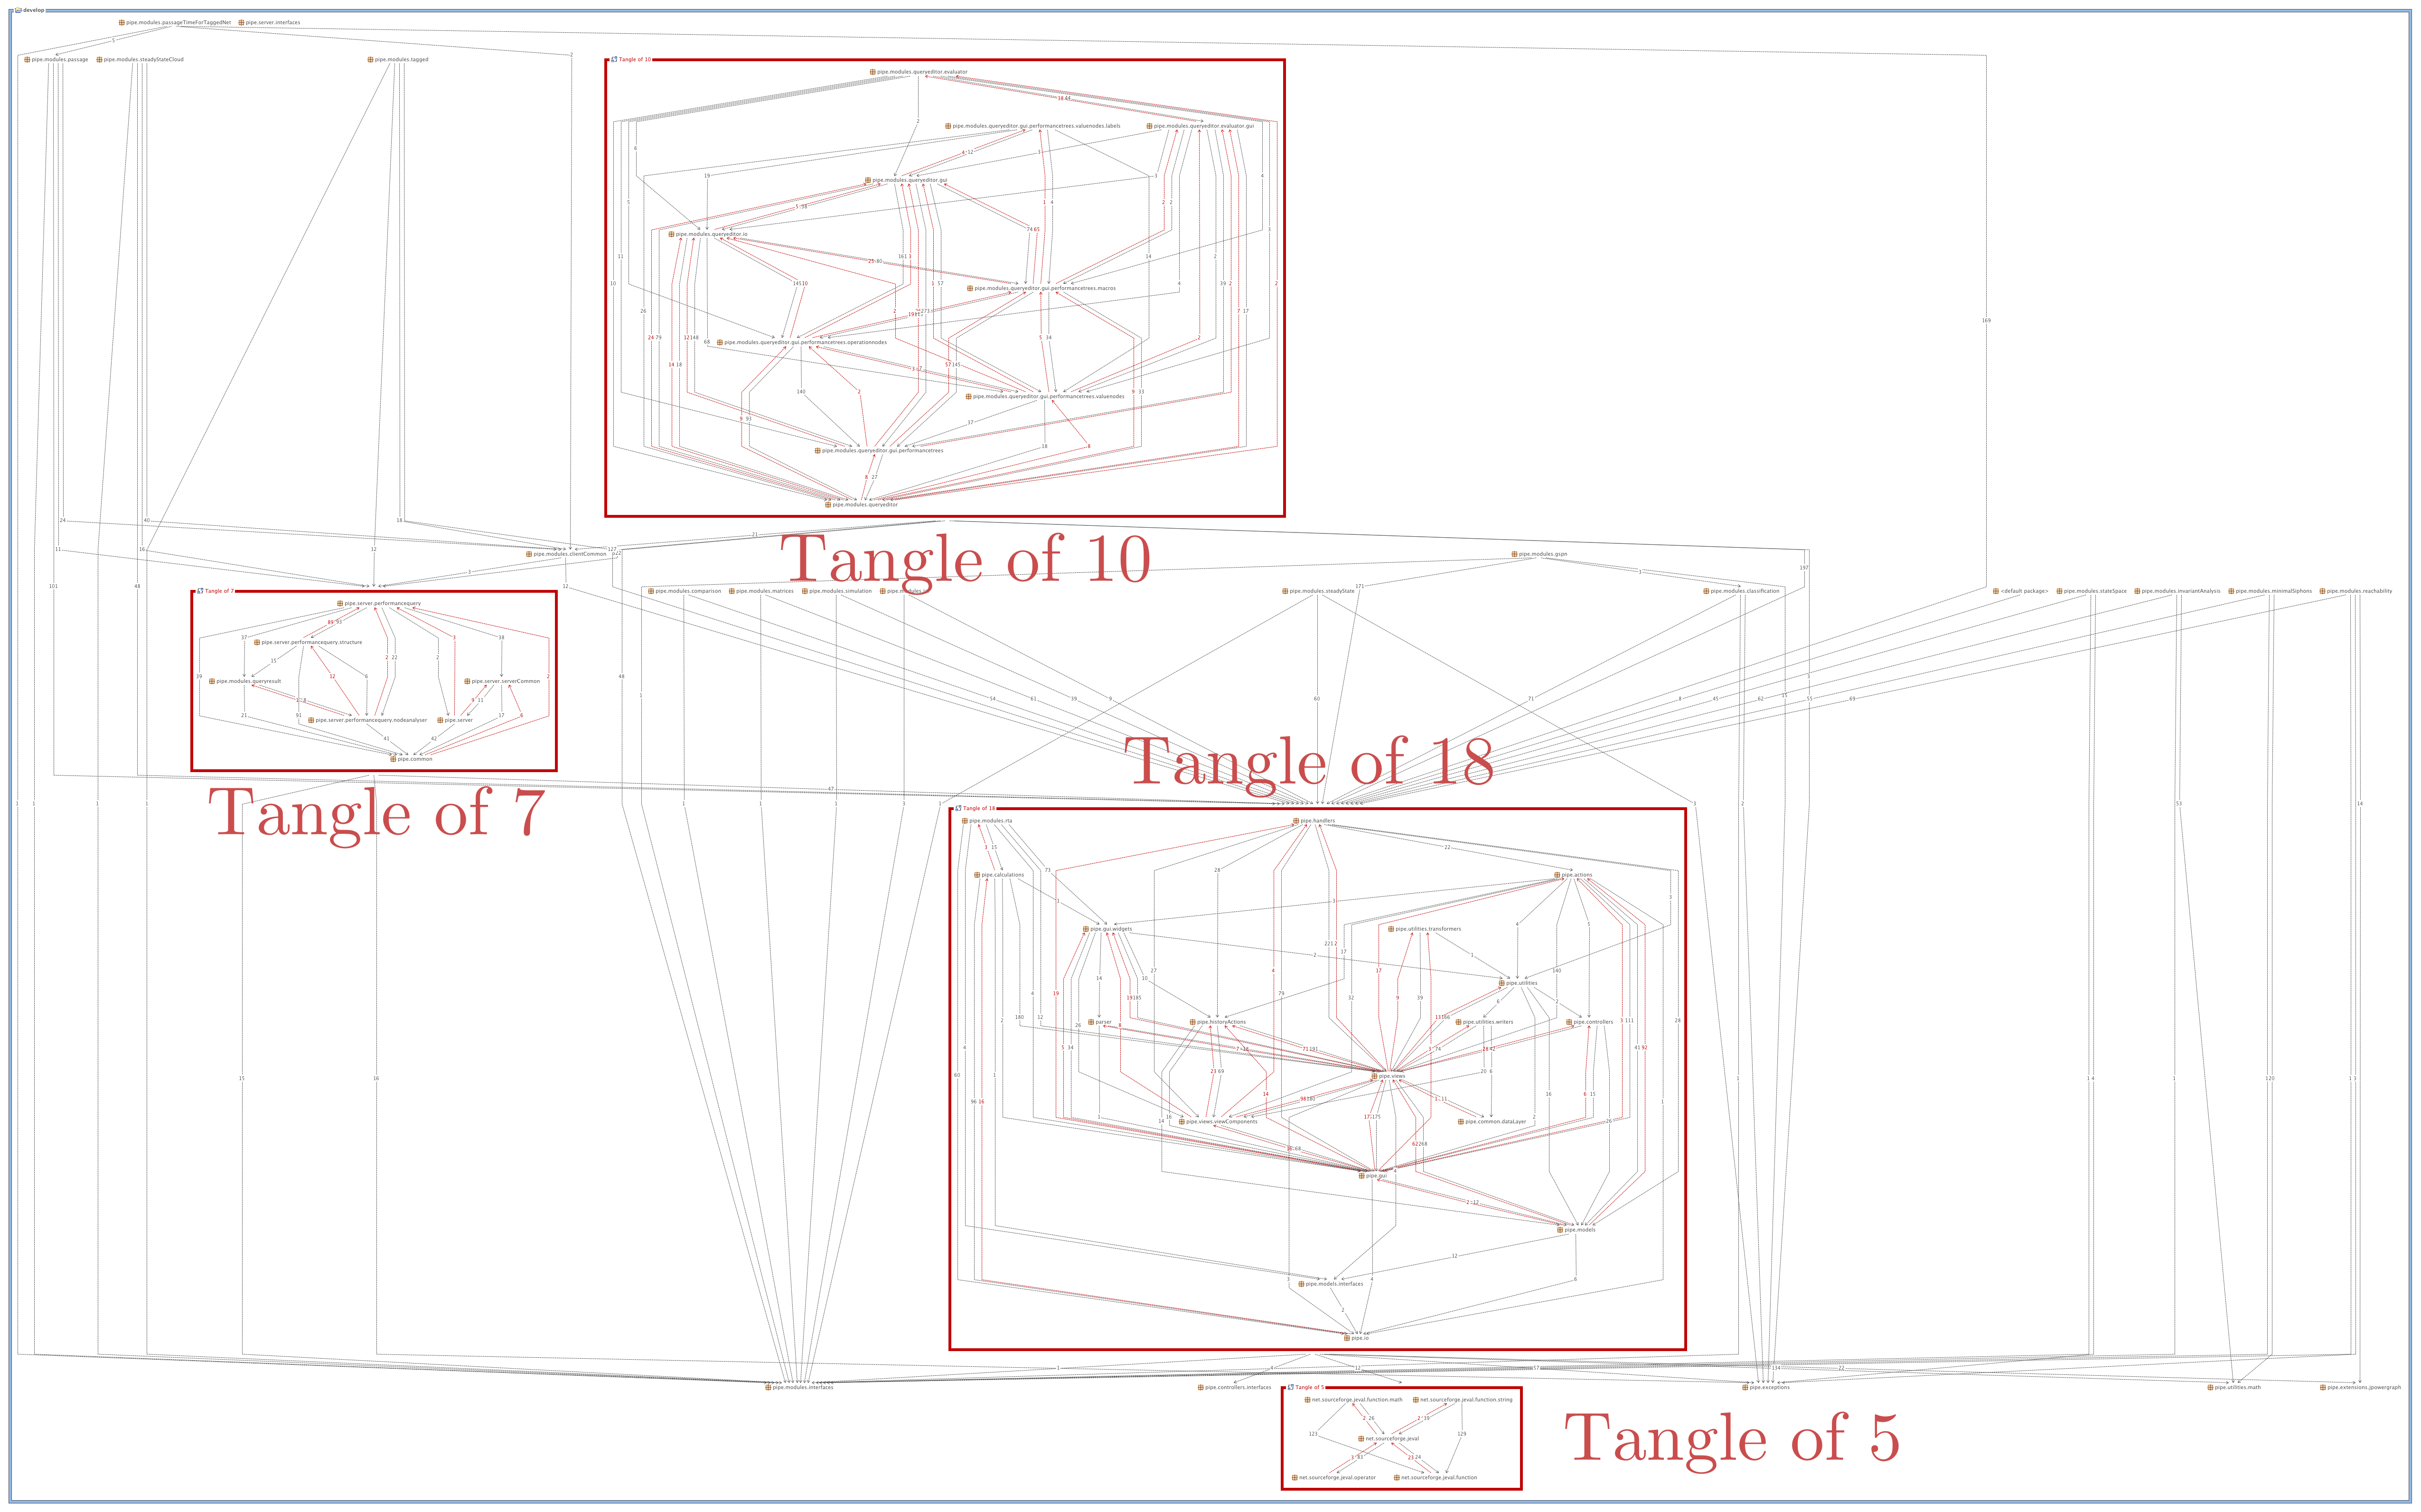
\includegraphics[width=\textwidth]{eval/original_tangle_annotated.png} 
}
\subcaptionbox{The tangle graph for the PIPE repository housing the view code in PIPE 5 which contains the Swing GUI code. It contains only a single tangle of size 11. Unfortunately due to time constraints PIPE 5 uses much of the original PIPE 4 architecture which is why we were not able to reduce the tangle count further as many of the existing classes are tightly coupled. }{
    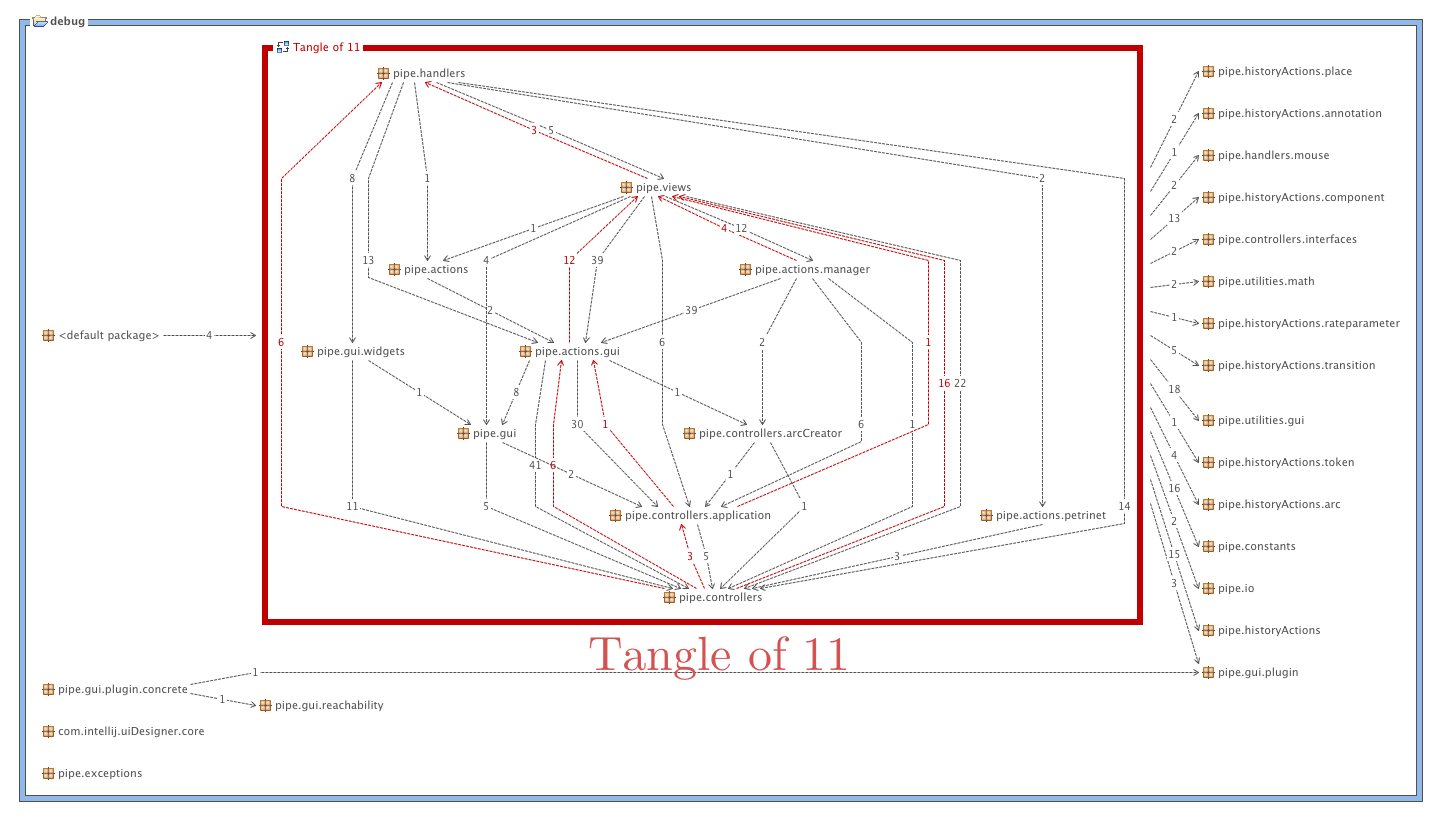
\includegraphics[width=\textwidth]{eval/gui_tangle_annotated.png} 
}
% \caption{Tangle results}
\label{fig:tangle_results}
\end{center}
\end{figure}
\begin{figure}[tbp]
\begin{center}
\ContinuedFloat
\subcaptionbox{The new PIPE 5 tangle graph for the PIPECore repository reporting a single tangle of size 2. This tangle is between the functional expression parsers and the Petri net models. It has been kept because it improves the quality of the API by allowing Petri net components, namely transitions, to be able to evaluate their functional expressions without extra interaction from the user.}{
    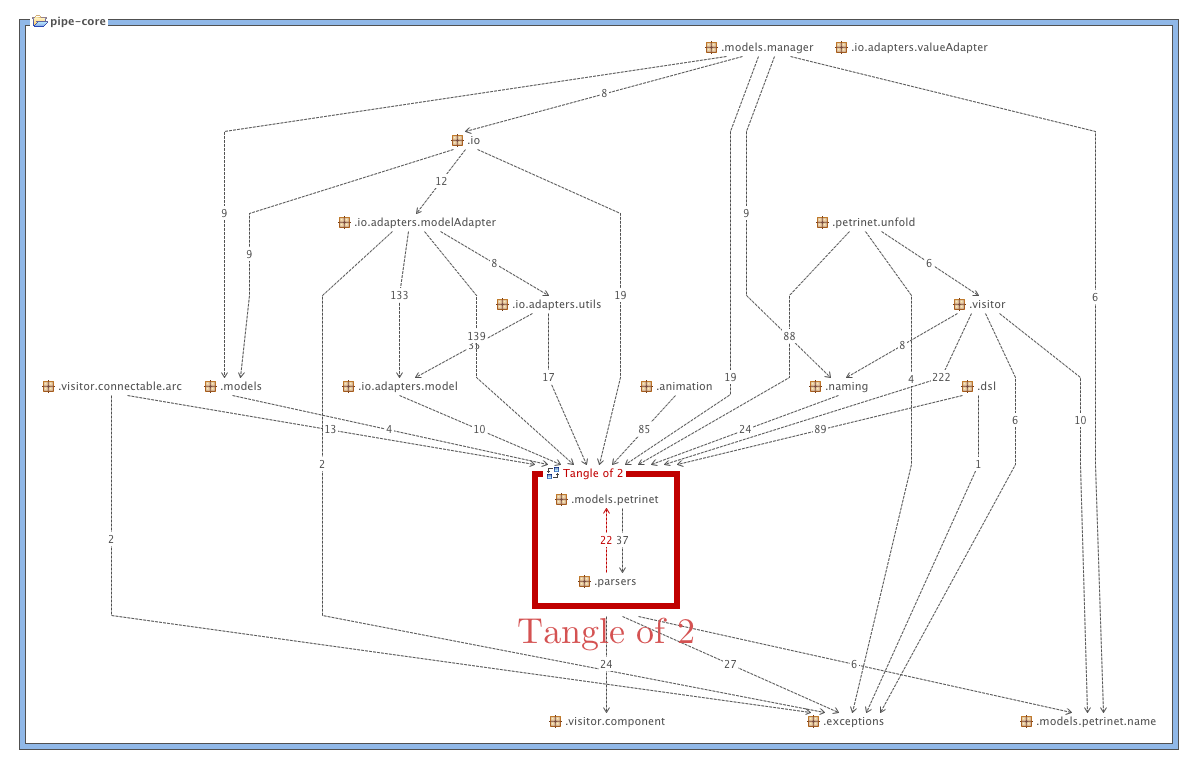
\includegraphics[width=\textwidth]{eval/pipe_core_tangle_annotated.png} 
}
\subcaptionbox{The tangle graph for the new PIPEAnalysis repository containing the code for the steady state solver and the state space exploration. It reports 0 tangles.}{
    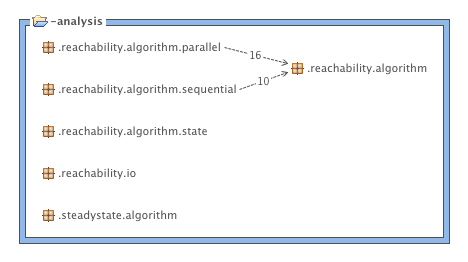
\includegraphics[scale=0.5]{eval/pipe_analysis_tangle.png} 
}
\hspace{5mm}
\subcaptionbox{The tangle graph for the new PIPEMarkovChain repository containing the classes which represent the underlying Markov chain of a Petri net and the explored sets data structure. It reports 0 tangles.}{
    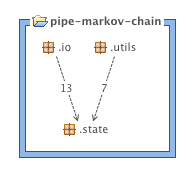
\includegraphics[scale=0.7]{eval/pipe_markov_chain_tangle.png} 
}
\caption{A comparison of the tangles in the PIPE 5 architecture against those in the PIPE 4 architecture. The tangle graphs clearly show a reduction from four tangles of size 18, 10, 7 and 5 down to only two tangles of size 11 and 2.}
\label{fig:tangle_results}
\end{center}
\end{figure}